\subsection{Confianza en los Resultados de la IA según Género de los estudiantes}
El análisis tiene como objetivo analizar los motivos por los cuales los encuestados emplean herramientas de inteligencia artificial. El objetivo es identificar el motivo predominante mediante el uso de medidas de tendencia central como la moda, la media y la mediana.\\

\textbf{Tabla de frecuencias:}
\begin{table}[H]
	\centering
	\renewcommand{\arraystretch}{1.2}
	\begin{tabular}{l c c c c}
		\hline
		{Respuesta} & {\(f_i\)} & \textit{Fi} & \textit{hi}(\%) & \textit{Hi}(\%)\\
		\hline
		Ahorrar tiempo        & 24 & 24 & 31.17\% & 31.17\%\\
		Obtener ideas         & 24 & 48 & 31.17\% & 62.34\%\\
		Resolver dudas        & 14 & 62 & 18.18\% & 80.52\%\\
		Simplificar conceptos & 9  & 71 & 11.69\% & 92.21\%\\
		Ampliar conocimientos & 6  & 77 & 7.79\%  & 100.0\%\\
		\hline
		Total                 & 77 &    & 100.0\%\\
		\hline
	\end{tabular}
	\caption{Distribución de respuestas sobre el uso de la I.A. para diferentes propósitos}
	\label{tabla:motivos}
\end{table}

\textbf{Media($\bar{x}$):} Dado que las categorías representan motivos cualitativos, se asignará marcas de clases como valores numéricos representativos:
\begin{itemize}
	\item “Ahorrar tiempo al hacer trabajos o investigaciones": 1
	\item "Obtener ideas y ejemplos": 2
	\item "Resolver dudas cuando no encuentro respuestas": 3
	\item "Simplificar conceptos complejos para entenderlos mejor": 4
	\item "Ampliar mi conocimiento sobre temas que no domino": 5
\end{itemize}
\begin{equation*}
	\bar{x} = \frac{\sum ()x_i . f_i)}{\sum f_i} = \frac{(1 . 24)+ (2 . 24) + (3 . 14) + (4 . 9) + (5 . 6)}{77} = \frac{180}{77} \approx 2.34
\end{equation*}
Esto indica que, en promedio, los encuestados seleccionaron una opción cercana a la segunda opción de la escala que corresponde a "Obtener ideas y ejemplos".

\textbf{Mediana($M_e$):} La mediana es el valor que se encuentra en el centro de la distribución de respuestas.
\begin{equation*}
	M_e = \frac{n + 1}{2} \approx 39
\end{equation*}
Esto se interpreta como que la mediana cae en la clase de “Obtener ideas y ejemplos”, representando el punto central de los datos.

\textbf{Moda($M_o$):}La moda es la categoría con la mayor frecuencia absoluta($f_i$), al compararlos se puede llegar a la conclusión que la moda de la distribución es bimodal, siendo las categorías “Ahorrar tiempo al hacer trabajos o investigaciones” y “Obtener ideas y ejemplos” las más seleccionadas por los encuestados, con una frecuencia de 24 respuestas cada una.
\begin{figure}[H]
	\centering
	\hspace*{-1.5cm}
	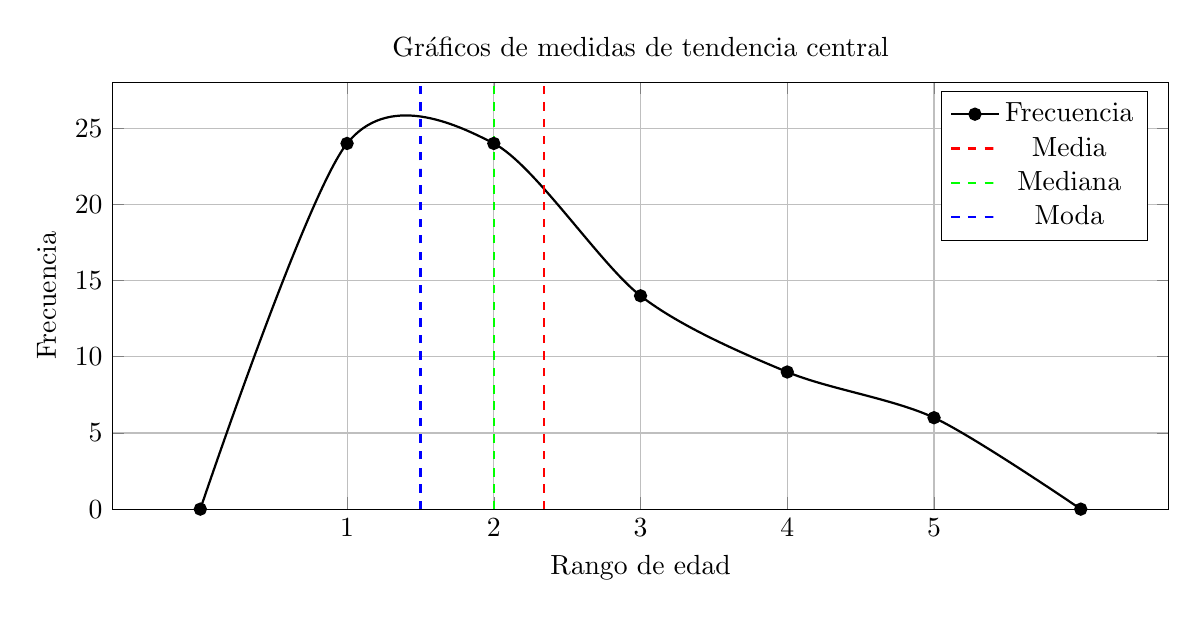
\begin{tikzpicture}
		\begin{axis}[
			width=15cm, height=7cm,
			xlabel={Rango de edad},
			ylabel={Frecuencia},
			xtick={1,2,3,4,5},
			extra x ticks={1.5, 1.99},
			ymin=0, ymax=28,
			grid=major,
			smooth,
			tension=0.5,
			extra tick style={opacity=0},
			title={Gráficos de medidas de tendencia central}
			]
			
			\addplot[
			mark=*,
			color=black,
			thick
			] coordinates {
				(0,0)
				(1,24) 
				(2,24) 
				(3,14)  
				(4,9) 
				(5,6)
				(6,0)
			};
			
			%Media
			\addplot[
			color=red,
			thick,
			dashed
			] coordinates {(2.34, 0) (2.34, 28)}; 
			%Mediana
			\addplot[
			color=green,
			thick,
			dashed
			] coordinates {(2, 0) (2, 28)};
			%Moda
			\addplot[
			color=blue,
			thick,
			dashed
			] coordinates {(1.5, 0) (1.5, 28)}; 
			\legend{Frecuencia, Media, Mediana, Moda}
		\end{axis}
	\end{tikzpicture}
	\caption{Gráfico de frecuencia con línea de tendencia}
\end{figure}

\textbf{Interpretación de datos:} Los motivos más comunes para usar IA son "Ahorrar tiempo" y "Obtener ideas", con 24 respuestas (45.25\%) cada uno. La media de 2.34 indica una preferencia por opciones intermedias, como la eficiencia y la creatividad. La mediana confirma que la opción de "Obtener ideas" es representativa de la mayoría de los encuestados, mostrando que los usuarios valoran tanto la productividad como el apoyo creativo que ofrece la IA.
